% !TEX encoding = UTF-8
% !TEX TS-program = pdflatex
% !TEX root = ../tesi.tex

%**************************************************************
\chapter{L'attività di stage all'interno della strategia aziendale}
\label{cap:processi-metodologie}
%**************************************************************
\intro{Introduzione al capitolo}\\
  In questo capitolo si andrà ad illustrare la propensione dell'azienda rispetto allo stage, indicando le attività con le relative tematiche che mi sono state proposte e come tali siano inserite all'interno della strategia aziendale\\

%**************************************************************
\section{Vantaggi aziendali}
\textit{Siav} da molti anni ha stretto un accordo con l'Università di Padova per quanto riguarda la propensione a svolgere attività di stage. È in continua ricerca di nuove figure da poter inserire all'interno del loro organigramma, soprattutto per quanto riguarda studenti o neo laureati.  Essendo un'azienda in forte crescita ed espansione, necessita costantemente di nuovo personale, ma soprattutto, di nuove idee e tecnologie da poter poi attuare all'interno dei propri prodotti. La maggior parte degli stage vengono avviati dal settore di Ricerca e Sviluppo proprio per soddisfare questa necessità; solitamente le attività di stage proposte comprendono un periodo di formazione iniziale per poter prendere dimestichezza con le nuove tecnologie che si andranno ad attuare, per poi metterle in pratica con il supporto costante del team. Questa sezione presente all'interno di \textit{Siav} garantisce una costante dedizione alla ricerca, non soffermandosi a ciò che è già presente all'interno dell'azienda, ma cercando di spaziare tra più tematiche in contemporanea, procedendo all'attivazione di più stage in ambiti diversi, spaziando quindi la ricerca su più fronti. L'azienda, inoltre, avendo stipulato un cospicuo numero di \textit{partnership} si ritrova spesso e volentieri far partecipare i propri dipendenti a diversi \textit{meeting} o seminari per quanto riguarda lo studio e approfondimento di nuove tecnologie emergenti o di tendenza. Tali aspetti vengono poi valutati dal team tramite un studio di fattibilità per poter verificare se le tematiche affrontate possono portare qualcosa di redditizio all'interno del contesto aziendale. Quest'ultime portano \textit{Siav} ad essere una delle realtà italiane più attive e propense alla ricerca e allo sviluppo.

\section{Introduzione al progetto}
\textit{Siav} attraverso i numerosi progetti di stage mira ad esplorare nuove tematiche e nuove opportunità tecnologiche che possano portare ad un miglioramento dei propri prodotti. Il progetto che mi è stato proposto mirava proprio al miglioramento di un loro applicativo. Lo scopo dello stage, è stato diviso in tre parti:
\begin{itemize}
	\item sviluppo di una libreria di \textit{process mining} per la pulizia di log degli eventi
	\item sviluppo di un'interfaccia \textit{frontend} che rispettasse le tematiche presenti all'interno della libreria
	\item sviluppo di \gls{stub} che simulino il comportamento del \textit{backend} per verificare il corretto funzionamento dell'interfaccia.
\end{itemize}
Tramite questo stage è stato possibile per \textit{Siav} migliorare uno dei propri prodotti che aveva perso la sua mantenibilià, essendo stato sviluppato da un piccolo team che ora non era più presente in azienda. Oltretutto la documentazione è risultata scarsa e di difficile comprensione; è stato quindi deciso di riscrivere l'applicativo da zero, cercando di mantenere le principali funzionalità, analizzando qualche aspetto critico che presenteva la vecchia architettura e cercando un'alternativa solida basandosi su nuove tecniche e tecnologie che all'epoca non erano state prese in considerazione. 
\subsection{Analisi del software attuale}
Durante la prima parte dello stage l'obiettivo è quello di analizzare le funzionalità e interfaccia legate al filtraggio dei log presente nell'applicativo in modo da poter individuare tutte le possibili funzionalità disponibili all'utente. Dopo una revisione completa ed approfondita dell'applicativo ne è emerso che dal punto di vista delle funzionalità l'applicativo non aveva nulla da invidiare rispetto ai più comuni software di \textit{process mining}, presentando tutte le principali funzionalità per la modellazione di log. Dal punto di vista della sua efficenza però, le cose andavano diversamente: tutto il sistema era gestito tramite chiamate sicrone; ciò comportava la presenza di lunghi tempi di attesa per ogni operazione che l'utente intendeva effettuare. Solamente per effettuare un'operazione di filtraggio, per un log della dimensione di qualche \textit{Megabyte}, era necessario un tempo di attesa che andava da 1 a 5 secondi. Il che può essere accettabile, se non fosse che in ambito \textit{process mining}, per poter gestire di un cospicuo numero di processi, vengono analizzati log che possono essere di gran lunga più corposi e impegnativi da analizzare per il sistema. Da ciò ne è scaturatia l'idea di una restaurazione dell'applicativo.

\subsection{Progettazione libreria in relazione all'architettura finale}
In seguito all'attività di analisi del vecchio applicativo, un obiettivo dello stage risiede nella progettazione di un libreria di filtraggio in grado di poter effettuare la principali operazioni di pulizia su log degli eventi. Tale libreria dovrà soddisfare alcuni requisiti fonadmentali:
\begin{itemize}
	\item dovrà essere mantenibile nel tempo, facendo uso quindi di oppurtuni principi cardine della Programmazione ad Oggetti e dovrà essere documentata in modo preciso, facendo sì che chiunque la analizzi in futuro per poter effettuare alcune modifiche possa apprendere in modo chiaro e trasparente ogni sua parte e la sua struttua.
	\item dovrà essere affidabile e testata in ogni sua parte tramite \textit{Unit Test} in modo da garantire una base solida di partenza per poi contestualizzarla all'interno di un'architettura a microservizi
\end{itemize}
\subsection{Progettazione interfaccia \textit{frontend}}
Successivamente all'implementazione della libreria sarà necessario progettare l'interfaccia \textit{fronted}; per quest'ultima sarà necessario avvalersi del loro vecchio applicativo \textit{Bipod}, per poi confrontarlo con la libreria sviluppata discutendo con il tutor eventuali modifiche in caso di discrepanze. Tale interfaccia sarà rivista in modo più preciso ed approfondito una volta terminata la libreria, avendo quindi una visuale più ampie delle funzionalità offerte. Inoltre dovrà essere sviluppata con un framework ed un linguaggio più attuale rispetto al vecchio software, inoltre è stata richiesta un'interfaccia più intuitiva e semplificata rispetto a quella presente sull'applicativo odierno.
\begin{figure}[!h] 
	\centering 
	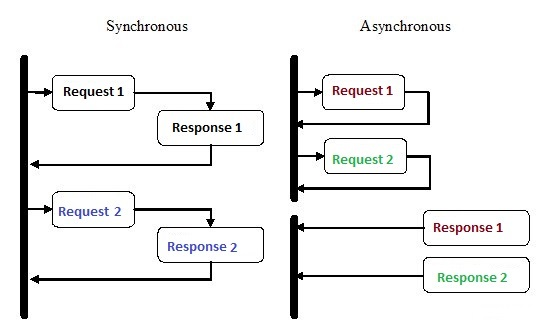
\includegraphics[width=1.0\columnwidth]{sync} 
	\caption{Illustazione della differenza tra chiamate sincrone ed asincrone}
\end{figure}
\newpage
\section{Aspettative aziendali}
Al termine delle 340 ore l'azienda si aspetta di avere un libreria di filtraggio solida ed estendibile, in grado di eseguire le principali funzionalità di filtraggio al'interno di un log degli eventi, un'interfaccia \textit{frontend} semplice ed intuitiva in grado di utilizzare tutte le funzionalità incluse all'interno della libreria e uno \textit{Stub} per osservare il comportamento di un'interfaccia, in relazione dell'architettura finale.
Il tutto deve essere pensato per un’erogazione in modalità \textit{cloud}, pertanto le scelte architetturali dovranno tener conto di questo prerequisito.
\begin{figure}[!h] 
	\centering 
	
\includegraphics[width=0.3\columnwidth]{cloud} 
	\caption{Illustazione semplificata di un'architettura server cloud (\url{https://www.volico.com/services/cloud-hosting/})}
\end{figure}
Tali attività mi hanno portato a definire i principali requisiti con il tutor aziendale, che sono poi stati inseriti all'interno del piano di lavoro. In seguito a ciò il tutor ha individuato gli obiettivi per il progetto suddividendoli in due categorie: obbligatori e desiderabili.\\
\\
\\
\begin{table}[!h]
	\caption{Obiettivi obbligatori dello stage}
\begin{tabularx}{\textwidth}{lXl}
	\hline\hline
	\textbf{Obiettivi obbligatori}\\
	\hline
	Inquadramento del problema: stesura di un documento di specifica del problema\\
	affrontato; &  \\
	\hline
	\hline
     Analisi dei requisiti e specifiche tecniche di progettazione: stesura dei relativi\\
     documenti; &  \\
	\hline
	\hline
	Implementazione del frontend web e dei servizi di backend necessari a gestire le\\
	funzionalità di filtraggio degli eventi &  \\
	\hline
	\hline
	Collaudo del sistema: il progetto deve prevedere una fase di test del software\\
	implementato, con documentazione dei risultati ottenuti &  \\
	\hline	
\end{tabularx}
\end{table}
\begin{table}[!h]
	\caption{Obiettivi desiderabili dello stage}
	\begin{tabularx}{\textwidth}{lXl}
		\hline\hline
		\textbf{Obiettivi desiderabili}\\
		\hline
		point-and-click sul processo per inserimento di filtri sulle successioni di eventi&  \\
		\hline
		\hline
		implementazione test frontend &  \\
		\hline
	\end{tabularx}
\end{table}
\subsection{Vincoli}
I vincoli che mi sono stati posti durante la stesura del piano di lavoro possono essere raggruppati in 3 categorie:
\subsubsection{Vincoli temporali}
Rappresentano i vincoli dal punto di vista del tempo. Lo svolgimento dello stage ha avuto una durata di 340 ore. Tali ore sono state dstribuite in modo uniforme durante l'arco di 9 settimane. Inizialmente sono state concordate 8 settimane, ma in seguito ad alcune criticità riscontrate in fase di sviluppo, con la conseguente negoziazione dei requisiti, sono state portate a 9; includendo quindi una settimana aggiuntiva per terminare tutte le attività concordate.
Nel periodo antecedente all'inizio dello stage l'azienda ha redatto una scansione temporale delle attività su base settimanale suddivisa nel seguente modo:
\begin{itemize}
	\item \textbf{Settimana 1}: Studio introduttivo del Process Mining con le relative tecnologie. Studio dell’architettura di storage messa a disposizione e del	framework ProM
	\item \textbf{Settimana 2}: Studio di fattibilità per la realizzazione dei moduli necessari a erogare le funzionalità di filtraggio
    \item \textbf{Settimana 3-4-5}: Progettazione dei moduli di discovery del processo, visualizzazione log e filtraggio
    \item \textbf{Settimana 6-7}: Implementazione del software e \textit{\gls{deploy}} su docker
    \item \textbf{Settimana 8}: Test e sperimentazione del software
\end{itemize}
Durante tutto il periodo sopraindicato è stata richiesta anche una documentazione sul lavoro, includendo una breve cronologia delle attività svolte, indicando le eventuali criticità riscontrate e specificando in che modo sono state affrontate e risolte.\\
Tale pianificazione è stata rinegoziata a partire dalla sesta settimana; in quanto l'architettura finale non era stata ancora ideata in modo specifico. Questo ha portato, in accordo con il tutor ad una rinegoziazione dei requisiti e quindi della attività programmate; sostituendo l'attività di \textit{deploy} su \textit{docker} con l'implmentazione di alcuni stub in modo da poter verificare il comportamento dell'interfaccia frontend.
\begin{figure}[!h] 
	\centering 
	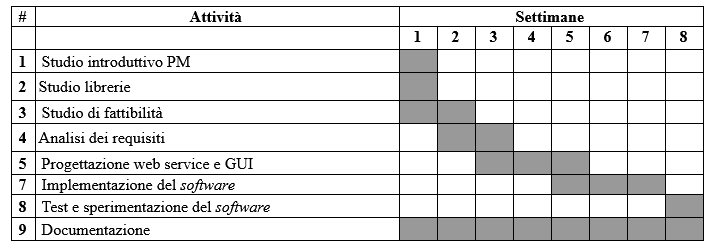
\includegraphics[width=1.0\columnwidth]{gantt} 
	\caption{Diagramma di gantt relativo alle attività di stage}
\end{figure}
\subsubsection{Vincoli metodologici}
Lo stage è stato svolto presso la sede di Rubano(PD) in comune accordo con il tutor. Ciò è stato deciso con lo scopo di poter confrantarsi ed interagire in maniera sistematica ogni qualvolta ce ne fosse stato bisogno; non soltanto tramite un rapporto stagista e tutor, ma confrontandosi con altri figure presenti all'interno dell'azienda in modo da poter consolidare nuovi rapporti di tipo professionale, in modo da avere supporto aggiuntivo in caso ce ne fosse stata necessità.
Oltre a ciò è stato richiesto un continuo confronto sulle attività effettuate e quelle in programma tramite alcune note di testo condivise tra il tutor ed il team di Ricerca e Sviluppo.
Tali note sono poi oggetto di discussione tramite \textit{Daily meeting}: in cui vi è un momento di confronto tra i membri del team per discutere in merito alle attività svolte e quelle in programma per la giornata. Mi è stata messa a disposizione una postazione di lavoro con personal computer, connessione ad Internet ed alla rete locale con accesso al server di sviluppo, in modo da poter effettuare \textit{deploy} di eventuali macchine virtuali necessarie allo sviluppo. Sono stati forniti una serie dati di esempio per testare quanto sviluppato, oltre a tutte le librerie necessarie allo sviluppo stesso dell’applicativo.
\begin{figure}[!h] 
	\centering 
	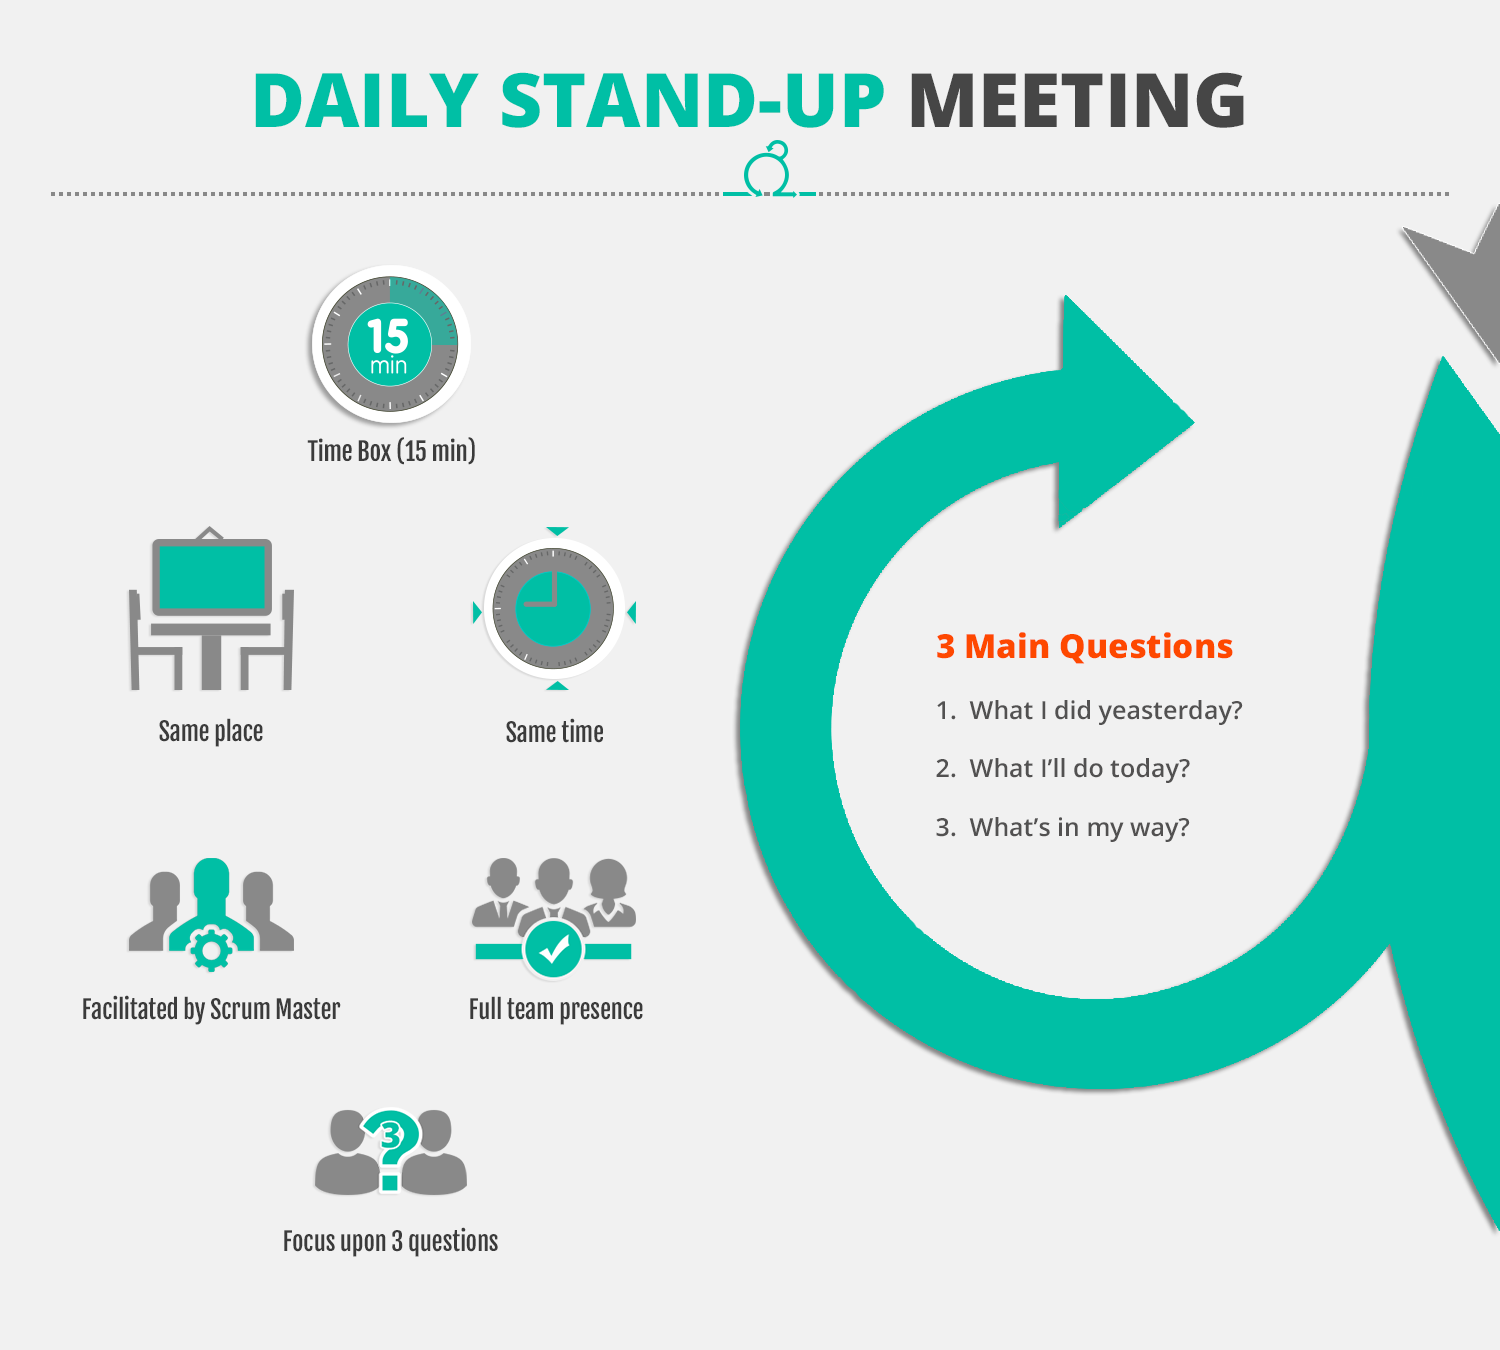
\includegraphics[width=0.95\columnwidth]{daily} 
	\caption{Illustrazione semplificata di \textit{Daily Meeting} (\url{https://tinyurl.com/ub822u3})}
\end{figure}
\subsubsection{Vincoli tecnologici}
Come sopra descritto l'obiettivo fondamentamentale per l'azienda è che l'applicativo finale fosse in grado di girare su server \textit{Cloud}. Questo ha influito in modo significativo sui vincoli tecnologici che sono stati imposti. Innanzitutto tramite lo sviluppo di una libreria che fosse scritta in modo semplice e leggibile, per far sì che chi dovrà inserirla nell'ambiente a microservizi abbia un'idea precisa delle sue caratterische ed il suo funzionamento; in secondo luogo tramite la gestione dell'asincronia all'interno dell'interfaccia \textit{frontend}, andando a gestire i messaggi in arrivo dal server, categorizzandoli e adattando il comportamente dell'interfaccia a seconda della caratterizzazione del messaggio in arrivo.
\section{Aspettative personali}
Tutte le mie passate esperienze sono riconducibili esclusivamento all'ambito accademico; l'esperienza che più mi ha avvicinato all'ambito lavorativo è stato il progetto di Ingegneria del Software; tramite il quale ho potuto constatare alcune dinamiche presenti all'interno di un contesto professionale. Per poter approcciarmi al mondo lavorativo ho partecipato all'evento organizzato dall'Università di Padova \textit{\gls{Stage-IT}}; tramite il quale ho potuto affrontare diversi incontri con realtà aziendali ben formate e strutturate. Durante la fiera ho potuto valutare diverse attività di stage tenendo in considerazione le tematiche trattate e quanto ciò potessero incidere nel mio grado di formazione. La maggior parte di esse però, non sono risultate, a mio parere, stimolanti per la mia maturità a livello professionale. 
Le aspettative che mi sono preposto prima dell'evento di \textit{Stage-IT} sono state le seguenti:
\begin{itemize}
	\item Introduzione a nuove metodologie di lavoro.
	\item Visione e apprendimento di nuove tecnologie.
	\item Lavoro in modo autonomo sotto la supervisione che tutor che mi presti supporto.
	\item Visione del contesto lavorativo in maniera più ampia, non legata strettamente all'attività di stage.
\end{itemize}
Successivamente a \textit{Stage-IT} sono stato contattato da altre aziende operanti nel settore dell'informatica, ognuna delle quali mi ha proposto varie attività affrontando diversi argomenti e tecnologie.
Una su tutte che mi ha colpito è stata proprio \textit{Siav} che, attraverso le loro proposte e la loro costante dedizione in merito alla ricerca di nuove tematiche e tecnologie mi ha convinto a svolgere l'attività di stage presso la loro azienda, collocandomi proprio all'interno del team di Ricerca e Sviluppo. Ciò ha comportato un aumento delle mie aspettative di fronte a questa attivita:
\begin{itemize}
	\item Valutare quanto possano essermi state utili le nozioni apprese durante il percorso universitario.
	\item Apprendimento dei principi cardine del process mining.
	\item Apprendimento sul funzionamento di un'architettura a microservizi.
	\item Instaurazione di discussioni con il personale dell'azienda in modo da potersi confrontare ed avere diversi punti di vista rispetto ad alcune tematiche.
	
\end{itemize}
